\documentclass[11pt]{article}

    \usepackage[breakable]{tcolorbox}
    \usepackage{parskip} % Stop auto-indenting (to mimic markdown behaviour)
    
    \usepackage{iftex}
    \ifPDFTeX
    	\usepackage[T1]{fontenc}
    	\usepackage{mathpazo}
    \else
    	\usepackage{fontspec}
    \fi

    % Basic figure setup, for now with no caption control since it's done
    % automatically by Pandoc (which extracts ![](path) syntax from Markdown).
    \usepackage{graphicx}
    % Maintain compatibility with old templates. Remove in nbconvert 6.0
    \let\Oldincludegraphics\includegraphics
    % Ensure that by default, figures have no caption (until we provide a
    % proper Figure object with a Caption API and a way to capture that
    % in the conversion process - todo).
    \usepackage{caption}
    \DeclareCaptionFormat{nocaption}{}
    \captionsetup{format=nocaption,aboveskip=0pt,belowskip=0pt}

    \usepackage[Export]{adjustbox} % Used to constrain images to a maximum size
    \adjustboxset{max size={0.9\linewidth}{0.9\paperheight}}
    \usepackage{float}
    \floatplacement{figure}{H} % forces figures to be placed at the correct location
    \usepackage{xcolor} % Allow colors to be defined
    \usepackage{enumerate} % Needed for markdown enumerations to work
    \usepackage{geometry} % Used to adjust the document margins
    \usepackage{amsmath} % Equations
    \usepackage{amssymb} % Equations
    \usepackage{textcomp} % defines textquotesingle
    % Hack from http://tex.stackexchange.com/a/47451/13684:
    \AtBeginDocument{%
        \def\PYZsq{\textquotesingle}% Upright quotes in Pygmentized code
    }
    \usepackage{upquote} % Upright quotes for verbatim code
    \usepackage{eurosym} % defines \euro
    \usepackage[mathletters]{ucs} % Extended unicode (utf-8) support
    \usepackage{fancyvrb} % verbatim replacement that allows latex
    \usepackage{grffile} % extends the file name processing of package graphics 
                         % to support a larger range
    \makeatletter % fix for grffile with XeLaTeX
    \def\Gread@@xetex#1{%
      \IfFileExists{"\Gin@base".bb}%
      {\Gread@eps{\Gin@base.bb}}%
      {\Gread@@xetex@aux#1}%
    }
    \makeatother

    % The hyperref package gives us a pdf with properly built
    % internal navigation ('pdf bookmarks' for the table of contents,
    % internal cross-reference links, web links for URLs, etc.)
    \usepackage{hyperref}
    % The default LaTeX title has an obnoxious amount of whitespace. By default,
    % titling removes some of it. It also provides customization options.
    \usepackage{titling}
    \usepackage{longtable} % longtable support required by pandoc >1.10
    \usepackage{booktabs}  % table support for pandoc > 1.12.2
    \usepackage[inline]{enumitem} % IRkernel/repr support (it uses the enumerate* environment)
    \usepackage[normalem]{ulem} % ulem is needed to support strikethroughs (\sout)
                                % normalem makes italics be italics, not underlines
    \usepackage{mathrsfs}
    

    
    % Colors for the hyperref package
    \definecolor{urlcolor}{rgb}{0,.145,.698}
    \definecolor{linkcolor}{rgb}{.71,0.21,0.01}
    \definecolor{citecolor}{rgb}{.12,.54,.11}

    % ANSI colors
    \definecolor{ansi-black}{HTML}{3E424D}
    \definecolor{ansi-black-intense}{HTML}{282C36}
    \definecolor{ansi-red}{HTML}{E75C58}
    \definecolor{ansi-red-intense}{HTML}{B22B31}
    \definecolor{ansi-green}{HTML}{00A250}
    \definecolor{ansi-green-intense}{HTML}{007427}
    \definecolor{ansi-yellow}{HTML}{DDB62B}
    \definecolor{ansi-yellow-intense}{HTML}{B27D12}
    \definecolor{ansi-blue}{HTML}{208FFB}
    \definecolor{ansi-blue-intense}{HTML}{0065CA}
    \definecolor{ansi-magenta}{HTML}{D160C4}
    \definecolor{ansi-magenta-intense}{HTML}{A03196}
    \definecolor{ansi-cyan}{HTML}{60C6C8}
    \definecolor{ansi-cyan-intense}{HTML}{258F8F}
    \definecolor{ansi-white}{HTML}{C5C1B4}
    \definecolor{ansi-white-intense}{HTML}{A1A6B2}
    \definecolor{ansi-default-inverse-fg}{HTML}{FFFFFF}
    \definecolor{ansi-default-inverse-bg}{HTML}{000000}

    % commands and environments needed by pandoc snippets
    % extracted from the output of `pandoc -s`
    \providecommand{\tightlist}{%
      \setlength{\itemsep}{0pt}\setlength{\parskip}{0pt}}
    \DefineVerbatimEnvironment{Highlighting}{Verbatim}{commandchars=\\\{\}}
    % Add ',fontsize=\small' for more characters per line
    \newenvironment{Shaded}{}{}
    \newcommand{\KeywordTok}[1]{\textcolor[rgb]{0.00,0.44,0.13}{\textbf{{#1}}}}
    \newcommand{\DataTypeTok}[1]{\textcolor[rgb]{0.56,0.13,0.00}{{#1}}}
    \newcommand{\DecValTok}[1]{\textcolor[rgb]{0.25,0.63,0.44}{{#1}}}
    \newcommand{\BaseNTok}[1]{\textcolor[rgb]{0.25,0.63,0.44}{{#1}}}
    \newcommand{\FloatTok}[1]{\textcolor[rgb]{0.25,0.63,0.44}{{#1}}}
    \newcommand{\CharTok}[1]{\textcolor[rgb]{0.25,0.44,0.63}{{#1}}}
    \newcommand{\StringTok}[1]{\textcolor[rgb]{0.25,0.44,0.63}{{#1}}}
    \newcommand{\CommentTok}[1]{\textcolor[rgb]{0.38,0.63,0.69}{\textit{{#1}}}}
    \newcommand{\OtherTok}[1]{\textcolor[rgb]{0.00,0.44,0.13}{{#1}}}
    \newcommand{\AlertTok}[1]{\textcolor[rgb]{1.00,0.00,0.00}{\textbf{{#1}}}}
    \newcommand{\FunctionTok}[1]{\textcolor[rgb]{0.02,0.16,0.49}{{#1}}}
    \newcommand{\RegionMarkerTok}[1]{{#1}}
    \newcommand{\ErrorTok}[1]{\textcolor[rgb]{1.00,0.00,0.00}{\textbf{{#1}}}}
    \newcommand{\NormalTok}[1]{{#1}}
    
    % Additional commands for more recent versions of Pandoc
    \newcommand{\ConstantTok}[1]{\textcolor[rgb]{0.53,0.00,0.00}{{#1}}}
    \newcommand{\SpecialCharTok}[1]{\textcolor[rgb]{0.25,0.44,0.63}{{#1}}}
    \newcommand{\VerbatimStringTok}[1]{\textcolor[rgb]{0.25,0.44,0.63}{{#1}}}
    \newcommand{\SpecialStringTok}[1]{\textcolor[rgb]{0.73,0.40,0.53}{{#1}}}
    \newcommand{\ImportTok}[1]{{#1}}
    \newcommand{\DocumentationTok}[1]{\textcolor[rgb]{0.73,0.13,0.13}{\textit{{#1}}}}
    \newcommand{\AnnotationTok}[1]{\textcolor[rgb]{0.38,0.63,0.69}{\textbf{\textit{{#1}}}}}
    \newcommand{\CommentVarTok}[1]{\textcolor[rgb]{0.38,0.63,0.69}{\textbf{\textit{{#1}}}}}
    \newcommand{\VariableTok}[1]{\textcolor[rgb]{0.10,0.09,0.49}{{#1}}}
    \newcommand{\ControlFlowTok}[1]{\textcolor[rgb]{0.00,0.44,0.13}{\textbf{{#1}}}}
    \newcommand{\OperatorTok}[1]{\textcolor[rgb]{0.40,0.40,0.40}{{#1}}}
    \newcommand{\BuiltInTok}[1]{{#1}}
    \newcommand{\ExtensionTok}[1]{{#1}}
    \newcommand{\PreprocessorTok}[1]{\textcolor[rgb]{0.74,0.48,0.00}{{#1}}}
    \newcommand{\AttributeTok}[1]{\textcolor[rgb]{0.49,0.56,0.16}{{#1}}}
    \newcommand{\InformationTok}[1]{\textcolor[rgb]{0.38,0.63,0.69}{\textbf{\textit{{#1}}}}}
    \newcommand{\WarningTok}[1]{\textcolor[rgb]{0.38,0.63,0.69}{\textbf{\textit{{#1}}}}}
    
    
    % Define a nice break command that doesn't care if a line doesn't already
    % exist.
    \def\br{\hspace*{\fill} \\* }
    % Math Jax compatibility definitions
    \def\gt{>}
    \def\lt{<}
    \let\Oldtex\TeX
    \let\Oldlatex\LaTeX
    \renewcommand{\TeX}{\textrm{\Oldtex}}
    \renewcommand{\LaTeX}{\textrm{\Oldlatex}}
    % Document parameters
    % Document title
    \title{Neural Networks}
    
    
    
    
    
% Pygments definitions
\makeatletter
\def\PY@reset{\let\PY@it=\relax \let\PY@bf=\relax%
    \let\PY@ul=\relax \let\PY@tc=\relax%
    \let\PY@bc=\relax \let\PY@ff=\relax}
\def\PY@tok#1{\csname PY@tok@#1\endcsname}
\def\PY@toks#1+{\ifx\relax#1\empty\else%
    \PY@tok{#1}\expandafter\PY@toks\fi}
\def\PY@do#1{\PY@bc{\PY@tc{\PY@ul{%
    \PY@it{\PY@bf{\PY@ff{#1}}}}}}}
\def\PY#1#2{\PY@reset\PY@toks#1+\relax+\PY@do{#2}}

\expandafter\def\csname PY@tok@w\endcsname{\def\PY@tc##1{\textcolor[rgb]{0.73,0.73,0.73}{##1}}}
\expandafter\def\csname PY@tok@c\endcsname{\let\PY@it=\textit\def\PY@tc##1{\textcolor[rgb]{0.25,0.50,0.50}{##1}}}
\expandafter\def\csname PY@tok@cp\endcsname{\def\PY@tc##1{\textcolor[rgb]{0.74,0.48,0.00}{##1}}}
\expandafter\def\csname PY@tok@k\endcsname{\let\PY@bf=\textbf\def\PY@tc##1{\textcolor[rgb]{0.00,0.50,0.00}{##1}}}
\expandafter\def\csname PY@tok@kp\endcsname{\def\PY@tc##1{\textcolor[rgb]{0.00,0.50,0.00}{##1}}}
\expandafter\def\csname PY@tok@kt\endcsname{\def\PY@tc##1{\textcolor[rgb]{0.69,0.00,0.25}{##1}}}
\expandafter\def\csname PY@tok@o\endcsname{\def\PY@tc##1{\textcolor[rgb]{0.40,0.40,0.40}{##1}}}
\expandafter\def\csname PY@tok@ow\endcsname{\let\PY@bf=\textbf\def\PY@tc##1{\textcolor[rgb]{0.67,0.13,1.00}{##1}}}
\expandafter\def\csname PY@tok@nb\endcsname{\def\PY@tc##1{\textcolor[rgb]{0.00,0.50,0.00}{##1}}}
\expandafter\def\csname PY@tok@nf\endcsname{\def\PY@tc##1{\textcolor[rgb]{0.00,0.00,1.00}{##1}}}
\expandafter\def\csname PY@tok@nc\endcsname{\let\PY@bf=\textbf\def\PY@tc##1{\textcolor[rgb]{0.00,0.00,1.00}{##1}}}
\expandafter\def\csname PY@tok@nn\endcsname{\let\PY@bf=\textbf\def\PY@tc##1{\textcolor[rgb]{0.00,0.00,1.00}{##1}}}
\expandafter\def\csname PY@tok@ne\endcsname{\let\PY@bf=\textbf\def\PY@tc##1{\textcolor[rgb]{0.82,0.25,0.23}{##1}}}
\expandafter\def\csname PY@tok@nv\endcsname{\def\PY@tc##1{\textcolor[rgb]{0.10,0.09,0.49}{##1}}}
\expandafter\def\csname PY@tok@no\endcsname{\def\PY@tc##1{\textcolor[rgb]{0.53,0.00,0.00}{##1}}}
\expandafter\def\csname PY@tok@nl\endcsname{\def\PY@tc##1{\textcolor[rgb]{0.63,0.63,0.00}{##1}}}
\expandafter\def\csname PY@tok@ni\endcsname{\let\PY@bf=\textbf\def\PY@tc##1{\textcolor[rgb]{0.60,0.60,0.60}{##1}}}
\expandafter\def\csname PY@tok@na\endcsname{\def\PY@tc##1{\textcolor[rgb]{0.49,0.56,0.16}{##1}}}
\expandafter\def\csname PY@tok@nt\endcsname{\let\PY@bf=\textbf\def\PY@tc##1{\textcolor[rgb]{0.00,0.50,0.00}{##1}}}
\expandafter\def\csname PY@tok@nd\endcsname{\def\PY@tc##1{\textcolor[rgb]{0.67,0.13,1.00}{##1}}}
\expandafter\def\csname PY@tok@s\endcsname{\def\PY@tc##1{\textcolor[rgb]{0.73,0.13,0.13}{##1}}}
\expandafter\def\csname PY@tok@sd\endcsname{\let\PY@it=\textit\def\PY@tc##1{\textcolor[rgb]{0.73,0.13,0.13}{##1}}}
\expandafter\def\csname PY@tok@si\endcsname{\let\PY@bf=\textbf\def\PY@tc##1{\textcolor[rgb]{0.73,0.40,0.53}{##1}}}
\expandafter\def\csname PY@tok@se\endcsname{\let\PY@bf=\textbf\def\PY@tc##1{\textcolor[rgb]{0.73,0.40,0.13}{##1}}}
\expandafter\def\csname PY@tok@sr\endcsname{\def\PY@tc##1{\textcolor[rgb]{0.73,0.40,0.53}{##1}}}
\expandafter\def\csname PY@tok@ss\endcsname{\def\PY@tc##1{\textcolor[rgb]{0.10,0.09,0.49}{##1}}}
\expandafter\def\csname PY@tok@sx\endcsname{\def\PY@tc##1{\textcolor[rgb]{0.00,0.50,0.00}{##1}}}
\expandafter\def\csname PY@tok@m\endcsname{\def\PY@tc##1{\textcolor[rgb]{0.40,0.40,0.40}{##1}}}
\expandafter\def\csname PY@tok@gh\endcsname{\let\PY@bf=\textbf\def\PY@tc##1{\textcolor[rgb]{0.00,0.00,0.50}{##1}}}
\expandafter\def\csname PY@tok@gu\endcsname{\let\PY@bf=\textbf\def\PY@tc##1{\textcolor[rgb]{0.50,0.00,0.50}{##1}}}
\expandafter\def\csname PY@tok@gd\endcsname{\def\PY@tc##1{\textcolor[rgb]{0.63,0.00,0.00}{##1}}}
\expandafter\def\csname PY@tok@gi\endcsname{\def\PY@tc##1{\textcolor[rgb]{0.00,0.63,0.00}{##1}}}
\expandafter\def\csname PY@tok@gr\endcsname{\def\PY@tc##1{\textcolor[rgb]{1.00,0.00,0.00}{##1}}}
\expandafter\def\csname PY@tok@ge\endcsname{\let\PY@it=\textit}
\expandafter\def\csname PY@tok@gs\endcsname{\let\PY@bf=\textbf}
\expandafter\def\csname PY@tok@gp\endcsname{\let\PY@bf=\textbf\def\PY@tc##1{\textcolor[rgb]{0.00,0.00,0.50}{##1}}}
\expandafter\def\csname PY@tok@go\endcsname{\def\PY@tc##1{\textcolor[rgb]{0.53,0.53,0.53}{##1}}}
\expandafter\def\csname PY@tok@gt\endcsname{\def\PY@tc##1{\textcolor[rgb]{0.00,0.27,0.87}{##1}}}
\expandafter\def\csname PY@tok@err\endcsname{\def\PY@bc##1{\setlength{\fboxsep}{0pt}\fcolorbox[rgb]{1.00,0.00,0.00}{1,1,1}{\strut ##1}}}
\expandafter\def\csname PY@tok@kc\endcsname{\let\PY@bf=\textbf\def\PY@tc##1{\textcolor[rgb]{0.00,0.50,0.00}{##1}}}
\expandafter\def\csname PY@tok@kd\endcsname{\let\PY@bf=\textbf\def\PY@tc##1{\textcolor[rgb]{0.00,0.50,0.00}{##1}}}
\expandafter\def\csname PY@tok@kn\endcsname{\let\PY@bf=\textbf\def\PY@tc##1{\textcolor[rgb]{0.00,0.50,0.00}{##1}}}
\expandafter\def\csname PY@tok@kr\endcsname{\let\PY@bf=\textbf\def\PY@tc##1{\textcolor[rgb]{0.00,0.50,0.00}{##1}}}
\expandafter\def\csname PY@tok@bp\endcsname{\def\PY@tc##1{\textcolor[rgb]{0.00,0.50,0.00}{##1}}}
\expandafter\def\csname PY@tok@fm\endcsname{\def\PY@tc##1{\textcolor[rgb]{0.00,0.00,1.00}{##1}}}
\expandafter\def\csname PY@tok@vc\endcsname{\def\PY@tc##1{\textcolor[rgb]{0.10,0.09,0.49}{##1}}}
\expandafter\def\csname PY@tok@vg\endcsname{\def\PY@tc##1{\textcolor[rgb]{0.10,0.09,0.49}{##1}}}
\expandafter\def\csname PY@tok@vi\endcsname{\def\PY@tc##1{\textcolor[rgb]{0.10,0.09,0.49}{##1}}}
\expandafter\def\csname PY@tok@vm\endcsname{\def\PY@tc##1{\textcolor[rgb]{0.10,0.09,0.49}{##1}}}
\expandafter\def\csname PY@tok@sa\endcsname{\def\PY@tc##1{\textcolor[rgb]{0.73,0.13,0.13}{##1}}}
\expandafter\def\csname PY@tok@sb\endcsname{\def\PY@tc##1{\textcolor[rgb]{0.73,0.13,0.13}{##1}}}
\expandafter\def\csname PY@tok@sc\endcsname{\def\PY@tc##1{\textcolor[rgb]{0.73,0.13,0.13}{##1}}}
\expandafter\def\csname PY@tok@dl\endcsname{\def\PY@tc##1{\textcolor[rgb]{0.73,0.13,0.13}{##1}}}
\expandafter\def\csname PY@tok@s2\endcsname{\def\PY@tc##1{\textcolor[rgb]{0.73,0.13,0.13}{##1}}}
\expandafter\def\csname PY@tok@sh\endcsname{\def\PY@tc##1{\textcolor[rgb]{0.73,0.13,0.13}{##1}}}
\expandafter\def\csname PY@tok@s1\endcsname{\def\PY@tc##1{\textcolor[rgb]{0.73,0.13,0.13}{##1}}}
\expandafter\def\csname PY@tok@mb\endcsname{\def\PY@tc##1{\textcolor[rgb]{0.40,0.40,0.40}{##1}}}
\expandafter\def\csname PY@tok@mf\endcsname{\def\PY@tc##1{\textcolor[rgb]{0.40,0.40,0.40}{##1}}}
\expandafter\def\csname PY@tok@mh\endcsname{\def\PY@tc##1{\textcolor[rgb]{0.40,0.40,0.40}{##1}}}
\expandafter\def\csname PY@tok@mi\endcsname{\def\PY@tc##1{\textcolor[rgb]{0.40,0.40,0.40}{##1}}}
\expandafter\def\csname PY@tok@il\endcsname{\def\PY@tc##1{\textcolor[rgb]{0.40,0.40,0.40}{##1}}}
\expandafter\def\csname PY@tok@mo\endcsname{\def\PY@tc##1{\textcolor[rgb]{0.40,0.40,0.40}{##1}}}
\expandafter\def\csname PY@tok@ch\endcsname{\let\PY@it=\textit\def\PY@tc##1{\textcolor[rgb]{0.25,0.50,0.50}{##1}}}
\expandafter\def\csname PY@tok@cm\endcsname{\let\PY@it=\textit\def\PY@tc##1{\textcolor[rgb]{0.25,0.50,0.50}{##1}}}
\expandafter\def\csname PY@tok@cpf\endcsname{\let\PY@it=\textit\def\PY@tc##1{\textcolor[rgb]{0.25,0.50,0.50}{##1}}}
\expandafter\def\csname PY@tok@c1\endcsname{\let\PY@it=\textit\def\PY@tc##1{\textcolor[rgb]{0.25,0.50,0.50}{##1}}}
\expandafter\def\csname PY@tok@cs\endcsname{\let\PY@it=\textit\def\PY@tc##1{\textcolor[rgb]{0.25,0.50,0.50}{##1}}}

\def\PYZbs{\char`\\}
\def\PYZus{\char`\_}
\def\PYZob{\char`\{}
\def\PYZcb{\char`\}}
\def\PYZca{\char`\^}
\def\PYZam{\char`\&}
\def\PYZlt{\char`\<}
\def\PYZgt{\char`\>}
\def\PYZsh{\char`\#}
\def\PYZpc{\char`\%}
\def\PYZdl{\char`\$}
\def\PYZhy{\char`\-}
\def\PYZsq{\char`\'}
\def\PYZdq{\char`\"}
\def\PYZti{\char`\~}
% for compatibility with earlier versions
\def\PYZat{@}
\def\PYZlb{[}
\def\PYZrb{]}
\makeatother


    % For linebreaks inside Verbatim environment from package fancyvrb. 
    \makeatletter
        \newbox\Wrappedcontinuationbox 
        \newbox\Wrappedvisiblespacebox 
        \newcommand*\Wrappedvisiblespace {\textcolor{red}{\textvisiblespace}} 
        \newcommand*\Wrappedcontinuationsymbol {\textcolor{red}{\llap{\tiny$\m@th\hookrightarrow$}}} 
        \newcommand*\Wrappedcontinuationindent {3ex } 
        \newcommand*\Wrappedafterbreak {\kern\Wrappedcontinuationindent\copy\Wrappedcontinuationbox} 
        % Take advantage of the already applied Pygments mark-up to insert 
        % potential linebreaks for TeX processing. 
        %        {, <, #, %, $, ' and ": go to next line. 
        %        _, }, ^, &, >, - and ~: stay at end of broken line. 
        % Use of \textquotesingle for straight quote. 
        \newcommand*\Wrappedbreaksatspecials {% 
            \def\PYGZus{\discretionary{\char`\_}{\Wrappedafterbreak}{\char`\_}}% 
            \def\PYGZob{\discretionary{}{\Wrappedafterbreak\char`\{}{\char`\{}}% 
            \def\PYGZcb{\discretionary{\char`\}}{\Wrappedafterbreak}{\char`\}}}% 
            \def\PYGZca{\discretionary{\char`\^}{\Wrappedafterbreak}{\char`\^}}% 
            \def\PYGZam{\discretionary{\char`\&}{\Wrappedafterbreak}{\char`\&}}% 
            \def\PYGZlt{\discretionary{}{\Wrappedafterbreak\char`\<}{\char`\<}}% 
            \def\PYGZgt{\discretionary{\char`\>}{\Wrappedafterbreak}{\char`\>}}% 
            \def\PYGZsh{\discretionary{}{\Wrappedafterbreak\char`\#}{\char`\#}}% 
            \def\PYGZpc{\discretionary{}{\Wrappedafterbreak\char`\%}{\char`\%}}% 
            \def\PYGZdl{\discretionary{}{\Wrappedafterbreak\char`\$}{\char`\$}}% 
            \def\PYGZhy{\discretionary{\char`\-}{\Wrappedafterbreak}{\char`\-}}% 
            \def\PYGZsq{\discretionary{}{\Wrappedafterbreak\textquotesingle}{\textquotesingle}}% 
            \def\PYGZdq{\discretionary{}{\Wrappedafterbreak\char`\"}{\char`\"}}% 
            \def\PYGZti{\discretionary{\char`\~}{\Wrappedafterbreak}{\char`\~}}% 
        } 
        % Some characters . , ; ? ! / are not pygmentized. 
        % This macro makes them "active" and they will insert potential linebreaks 
        \newcommand*\Wrappedbreaksatpunct {% 
            \lccode`\~`\.\lowercase{\def~}{\discretionary{\hbox{\char`\.}}{\Wrappedafterbreak}{\hbox{\char`\.}}}% 
            \lccode`\~`\,\lowercase{\def~}{\discretionary{\hbox{\char`\,}}{\Wrappedafterbreak}{\hbox{\char`\,}}}% 
            \lccode`\~`\;\lowercase{\def~}{\discretionary{\hbox{\char`\;}}{\Wrappedafterbreak}{\hbox{\char`\;}}}% 
            \lccode`\~`\:\lowercase{\def~}{\discretionary{\hbox{\char`\:}}{\Wrappedafterbreak}{\hbox{\char`\:}}}% 
            \lccode`\~`\?\lowercase{\def~}{\discretionary{\hbox{\char`\?}}{\Wrappedafterbreak}{\hbox{\char`\?}}}% 
            \lccode`\~`\!\lowercase{\def~}{\discretionary{\hbox{\char`\!}}{\Wrappedafterbreak}{\hbox{\char`\!}}}% 
            \lccode`\~`\/\lowercase{\def~}{\discretionary{\hbox{\char`\/}}{\Wrappedafterbreak}{\hbox{\char`\/}}}% 
            \catcode`\.\active
            \catcode`\,\active 
            \catcode`\;\active
            \catcode`\:\active
            \catcode`\?\active
            \catcode`\!\active
            \catcode`\/\active 
            \lccode`\~`\~ 	
        }
    \makeatother

    \let\OriginalVerbatim=\Verbatim
    \makeatletter
    \renewcommand{\Verbatim}[1][1]{%
        %\parskip\z@skip
        \sbox\Wrappedcontinuationbox {\Wrappedcontinuationsymbol}%
        \sbox\Wrappedvisiblespacebox {\FV@SetupFont\Wrappedvisiblespace}%
        \def\FancyVerbFormatLine ##1{\hsize\linewidth
            \vtop{\raggedright\hyphenpenalty\z@\exhyphenpenalty\z@
                \doublehyphendemerits\z@\finalhyphendemerits\z@
                \strut ##1\strut}%
        }%
        % If the linebreak is at a space, the latter will be displayed as visible
        % space at end of first line, and a continuation symbol starts next line.
        % Stretch/shrink are however usually zero for typewriter font.
        \def\FV@Space {%
            \nobreak\hskip\z@ plus\fontdimen3\font minus\fontdimen4\font
            \discretionary{\copy\Wrappedvisiblespacebox}{\Wrappedafterbreak}
            {\kern\fontdimen2\font}%
        }%
        
        % Allow breaks at special characters using \PYG... macros.
        \Wrappedbreaksatspecials
        % Breaks at punctuation characters . , ; ? ! and / need catcode=\active 	
        \OriginalVerbatim[#1,codes*=\Wrappedbreaksatpunct]%
    }
    \makeatother

    % Exact colors from NB
    \definecolor{incolor}{HTML}{303F9F}
    \definecolor{outcolor}{HTML}{D84315}
    \definecolor{cellborder}{HTML}{CFCFCF}
    \definecolor{cellbackground}{HTML}{F7F7F7}
    
    % prompt
    \makeatletter
    \newcommand{\boxspacing}{\kern\kvtcb@left@rule\kern\kvtcb@boxsep}
    \makeatother
    \newcommand{\prompt}[4]{
        \ttfamily\llap{{\color{#2}[#3]:\hspace{3pt}#4}}\vspace{-\baselineskip}
    }
    

    
    % Prevent overflowing lines due to hard-to-break entities
    \sloppy 
    % Setup hyperref package
    \hypersetup{
      breaklinks=true,  % so long urls are correctly broken across lines
      colorlinks=true,
      urlcolor=urlcolor,
      linkcolor=linkcolor,
      citecolor=citecolor,
      }
    % Slightly bigger margins than the latex defaults
    
    \geometry{verbose,tmargin=1in,bmargin=1in,lmargin=1in,rmargin=1in}
    
    

\begin{document}
    
    \maketitle
    
    

    
    Table of Contents{}

{{1~~}Dense layers}

{{1.1~~}{[}note-1{]} The linear regression model}

{{1.2~~}{[}note-2{]} What is a neural network?}

{{1.3~~}{[}code-1{]} A simple dense layer}

{{1.4~~}{[}code-2{]} Defining a complete model}

{{1.5~~}{[}note-3{]} High-level versus low-level approach}

{{1.6~~}{[}task-1{]} The linear algebra of dense layers}

{{1.7~~}{[}task-2{]} The low-level approach with multiple examples}

{{1.8~~}{[}task-3{]} Using the dense layer operation}

{{2~~}Requirements}

    \hypertarget{dense-layers}{%
\section{Dense layers}\label{dense-layers}}

    \hypertarget{note-1-the-linear-regression-model}{%
\subsection{\texorpdfstring{\texttt{{[}note-1{]}} The linear regression
model}{{[}note-1{]} The linear regression model}}\label{note-1-the-linear-regression-model}}

\begin{figure}
\centering
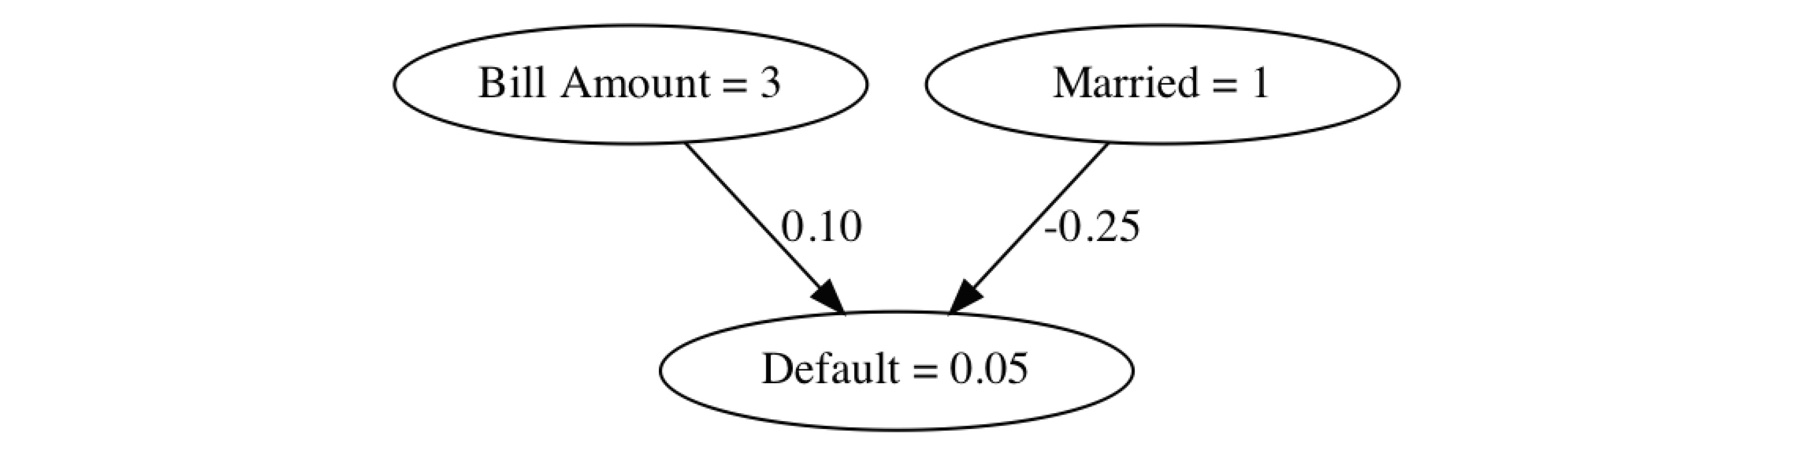
\includegraphics{../Figures/1. The linear regression model.jpg}
\caption{The linear regression model}
\end{figure}

    \hypertarget{note-2-what-is-a-neural-network}{%
\subsection{\texorpdfstring{\texttt{{[}note-2{]}} What is a neural
network?}{{[}note-2{]} What is a neural network?}}\label{note-2-what-is-a-neural-network}}

\begin{itemize}
\tightlist
\item
  A dense layer applies weights to all nodes from the previous layer.
\end{itemize}

\begin{figure}
\centering
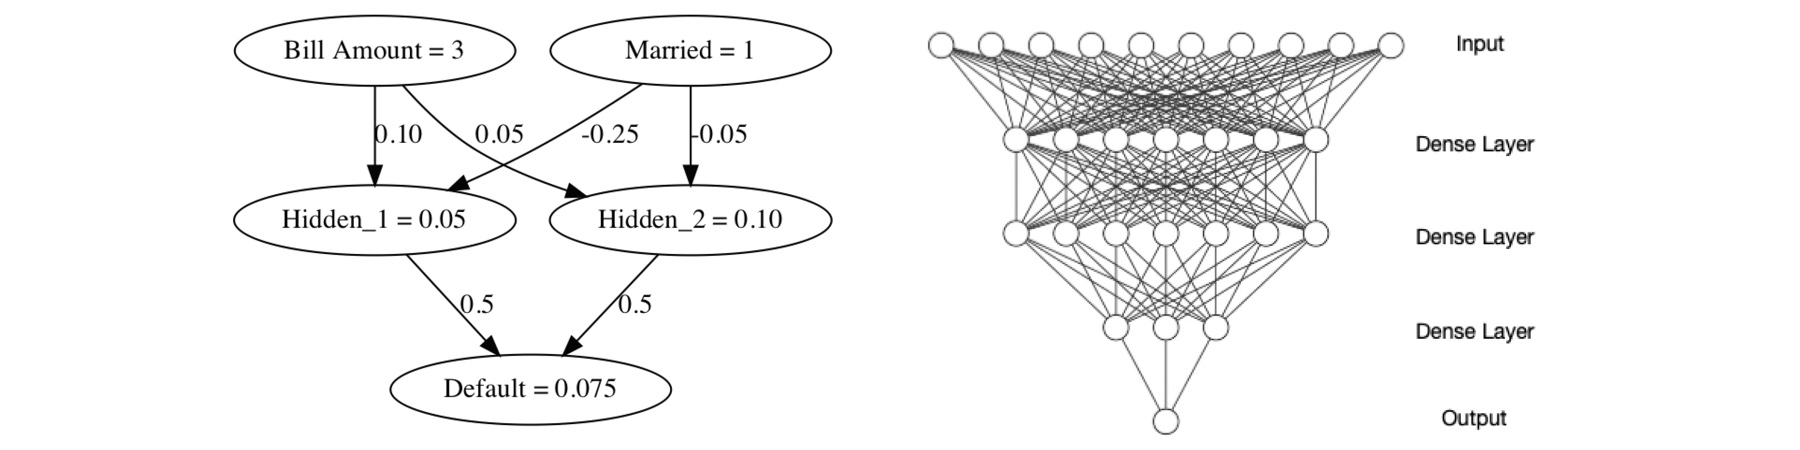
\includegraphics{../Figures/2. What is a neural network.jpg}
\caption{What is a neural network}
\end{figure}

    \hypertarget{code-1-a-simple-dense-layer}{%
\subsection{\texorpdfstring{\texttt{{[}code-1{]}} A simple dense
layer}{{[}code-1{]} A simple dense layer}}\label{code-1-a-simple-dense-layer}}

\begin{figure}
\centering

\includegraphics{../Figures/3. A simple dense layer.jpg}
\caption{A simple dense layer}
\end{figure}

    \begin{tcolorbox}[breakable, size=fbox, boxrule=1pt, pad at break*=1mm,colback=cellbackground, colframe=cellborder]
\prompt{In}{incolor}{28}{\boxspacing}
\begin{Verbatim}[commandchars=\\\{\}]
\PY{k+kn}{import} \PY{n+nn}{tensorflow} \PY{k}{as} \PY{n+nn}{tf}
\end{Verbatim}
\end{tcolorbox}

    \begin{tcolorbox}[breakable, size=fbox, boxrule=1pt, pad at break*=1mm,colback=cellbackground, colframe=cellborder]
\prompt{In}{incolor}{29}{\boxspacing}
\begin{Verbatim}[commandchars=\\\{\}]
\PY{c+c1}{\PYZsh{} Define inputs (features)}
\PY{n}{inputs} \PY{o}{=} \PY{n}{tf}\PY{o}{.}\PY{n}{constant}\PY{p}{(}\PY{p}{[}\PY{p}{[}\PY{l+m+mi}{1}\PY{p}{,} \PY{l+m+mi}{35}\PY{p}{]}\PY{p}{]}\PY{p}{,} \PY{n}{tf}\PY{o}{.}\PY{n}{float32}\PY{p}{)}
\end{Verbatim}
\end{tcolorbox}

    \begin{tcolorbox}[breakable, size=fbox, boxrule=1pt, pad at break*=1mm,colback=cellbackground, colframe=cellborder]
\prompt{In}{incolor}{30}{\boxspacing}
\begin{Verbatim}[commandchars=\\\{\}]
\PY{c+c1}{\PYZsh{} Define weights}
\PY{n}{weights} \PY{o}{=} \PY{n}{tf}\PY{o}{.}\PY{n}{Variable}\PY{p}{(}\PY{p}{[}\PY{p}{[}\PY{o}{\PYZhy{}}\PY{l+m+mf}{0.05}\PY{p}{]}\PY{p}{,} \PY{p}{[}\PY{o}{\PYZhy{}}\PY{l+m+mf}{0.01}\PY{p}{]}\PY{p}{]}\PY{p}{)}
\end{Verbatim}
\end{tcolorbox}

    \begin{tcolorbox}[breakable, size=fbox, boxrule=1pt, pad at break*=1mm,colback=cellbackground, colframe=cellborder]
\prompt{In}{incolor}{31}{\boxspacing}
\begin{Verbatim}[commandchars=\\\{\}]
\PY{c+c1}{\PYZsh{} Define the bias}
\PY{n}{bias} \PY{o}{=} \PY{n}{tf}\PY{o}{.}\PY{n}{Variable}\PY{p}{(}\PY{p}{[}\PY{l+m+mf}{0.5}\PY{p}{]}\PY{p}{)}
\end{Verbatim}
\end{tcolorbox}

    \begin{tcolorbox}[breakable, size=fbox, boxrule=1pt, pad at break*=1mm,colback=cellbackground, colframe=cellborder]
\prompt{In}{incolor}{32}{\boxspacing}
\begin{Verbatim}[commandchars=\\\{\}]
\PY{c+c1}{\PYZsh{} Multiply inputs (features) by the weights}
\PY{n}{product} \PY{o}{=} \PY{n}{tf}\PY{o}{.}\PY{n}{matmul}\PY{p}{(}\PY{n}{inputs}\PY{p}{,} \PY{n}{weights}\PY{p}{)}

\PY{n}{product}
\end{Verbatim}
\end{tcolorbox}

            \begin{tcolorbox}[breakable, size=fbox, boxrule=.5pt, pad at break*=1mm, opacityfill=0]
\prompt{Out}{outcolor}{32}{\boxspacing}
\begin{Verbatim}[commandchars=\\\{\}]
<tf.Tensor: shape=(1, 1), dtype=float32, numpy=array([[-0.4]], dtype=float32)>
\end{Verbatim}
\end{tcolorbox}
        
    \begin{tcolorbox}[breakable, size=fbox, boxrule=1pt, pad at break*=1mm,colback=cellbackground, colframe=cellborder]
\prompt{In}{incolor}{21}{\boxspacing}
\begin{Verbatim}[commandchars=\\\{\}]
\PY{c+c1}{\PYZsh{} Define dense layer}
\PY{n}{dense} \PY{o}{=} \PY{n}{tf}\PY{o}{.}\PY{n}{keras}\PY{o}{.}\PY{n}{activations}\PY{o}{.}\PY{n}{sigmoid}\PY{p}{(}\PY{n}{product} \PY{o}{+} \PY{n}{bias}\PY{p}{)}

\PY{n}{dense}
\end{Verbatim}
\end{tcolorbox}

            \begin{tcolorbox}[breakable, size=fbox, boxrule=.5pt, pad at break*=1mm, opacityfill=0]
\prompt{Out}{outcolor}{21}{\boxspacing}
\begin{Verbatim}[commandchars=\\\{\}]
<tf.Tensor: shape=(1, 1), dtype=float32, numpy=array([[0.5249792]],
dtype=float32)>
\end{Verbatim}
\end{tcolorbox}
        
    \hypertarget{code-2-defining-a-complete-model}{%
\subsection{\texorpdfstring{\texttt{{[}code-2{]}} Defining a complete
model}{{[}code-2{]} Defining a complete model}}\label{code-2-defining-a-complete-model}}

\begin{figure}
\centering

\includegraphics{../Figures/4. Defining a complete model.jpg}
\caption{Defining a complete model}
\end{figure}

    \begin{tcolorbox}[breakable, size=fbox, boxrule=1pt, pad at break*=1mm,colback=cellbackground, colframe=cellborder]
\prompt{In}{incolor}{22}{\boxspacing}
\begin{Verbatim}[commandchars=\\\{\}]
\PY{k+kn}{import} \PY{n+nn}{pandas} \PY{k}{as} \PY{n+nn}{pd}
\PY{k+kn}{import} \PY{n+nn}{tensorflow} \PY{k}{as} \PY{n+nn}{tf}

\PY{n}{data} \PY{o}{=} \PY{n}{pd}\PY{o}{.}\PY{n}{read\PYZus{}csv}\PY{p}{(}\PY{l+s+s2}{\PYZdq{}}\PY{l+s+s2}{../Datasets/1. Borrower features.csv}\PY{l+s+s2}{\PYZdq{}}\PY{p}{,} \PY{n}{header}\PY{o}{=}\PY{k+kc}{None}\PY{p}{)}
\end{Verbatim}
\end{tcolorbox}

    \begin{tcolorbox}[breakable, size=fbox, boxrule=1pt, pad at break*=1mm,colback=cellbackground, colframe=cellborder]
\prompt{In}{incolor}{24}{\boxspacing}
\begin{Verbatim}[commandchars=\\\{\}]
\PY{c+c1}{\PYZsh{} Define input (features) layer}
\PY{n}{inputs} \PY{o}{=} \PY{n}{tf}\PY{o}{.}\PY{n}{constant}\PY{p}{(}\PY{n}{data}\PY{p}{,} \PY{n}{tf}\PY{o}{.}\PY{n}{float32}\PY{p}{)}

\PY{n}{inputs}\PY{o}{.}\PY{n}{shape}
\end{Verbatim}
\end{tcolorbox}

            \begin{tcolorbox}[breakable, size=fbox, boxrule=.5pt, pad at break*=1mm, opacityfill=0]
\prompt{Out}{outcolor}{24}{\boxspacing}
\begin{Verbatim}[commandchars=\\\{\}]
TensorShape([100, 10])
\end{Verbatim}
\end{tcolorbox}
        
    \begin{tcolorbox}[breakable, size=fbox, boxrule=1pt, pad at break*=1mm,colback=cellbackground, colframe=cellborder]
\prompt{In}{incolor}{25}{\boxspacing}
\begin{Verbatim}[commandchars=\\\{\}]
\PY{c+c1}{\PYZsh{} Define first dense layer}
\PY{n}{dense1} \PY{o}{=} \PY{n}{tf}\PY{o}{.}\PY{n}{keras}\PY{o}{.}\PY{n}{layers}\PY{o}{.}\PY{n}{Dense}\PY{p}{(}\PY{l+m+mi}{10}\PY{p}{,} \PY{n}{activation}\PY{o}{=}\PY{l+s+s1}{\PYZsq{}}\PY{l+s+s1}{sigmoid}\PY{l+s+s1}{\PYZsq{}}\PY{p}{)}\PY{p}{(}\PY{n}{inputs}\PY{p}{)}

\PY{n}{dense1}\PY{o}{.}\PY{n}{shape}
\end{Verbatim}
\end{tcolorbox}

            \begin{tcolorbox}[breakable, size=fbox, boxrule=.5pt, pad at break*=1mm, opacityfill=0]
\prompt{Out}{outcolor}{25}{\boxspacing}
\begin{Verbatim}[commandchars=\\\{\}]
TensorShape([100, 10])
\end{Verbatim}
\end{tcolorbox}
        
    \begin{tcolorbox}[breakable, size=fbox, boxrule=1pt, pad at break*=1mm,colback=cellbackground, colframe=cellborder]
\prompt{In}{incolor}{26}{\boxspacing}
\begin{Verbatim}[commandchars=\\\{\}]
\PY{c+c1}{\PYZsh{} Define second dense layer}
\PY{n}{dense2} \PY{o}{=} \PY{n}{tf}\PY{o}{.}\PY{n}{keras}\PY{o}{.}\PY{n}{layers}\PY{o}{.}\PY{n}{Dense}\PY{p}{(}\PY{l+m+mi}{5}\PY{p}{,} \PY{n}{activation}\PY{o}{=}\PY{l+s+s1}{\PYZsq{}}\PY{l+s+s1}{sigmoid}\PY{l+s+s1}{\PYZsq{}}\PY{p}{)}\PY{p}{(}\PY{n}{dense1}\PY{p}{)}

\PY{n}{dense2}\PY{o}{.}\PY{n}{shape}
\end{Verbatim}
\end{tcolorbox}

            \begin{tcolorbox}[breakable, size=fbox, boxrule=.5pt, pad at break*=1mm, opacityfill=0]
\prompt{Out}{outcolor}{26}{\boxspacing}
\begin{Verbatim}[commandchars=\\\{\}]
TensorShape([100, 5])
\end{Verbatim}
\end{tcolorbox}
        
    \begin{tcolorbox}[breakable, size=fbox, boxrule=1pt, pad at break*=1mm,colback=cellbackground, colframe=cellborder]
\prompt{In}{incolor}{27}{\boxspacing}
\begin{Verbatim}[commandchars=\\\{\}]
\PY{c+c1}{\PYZsh{} Define output (predictions) layer}
\PY{n}{outputs} \PY{o}{=} \PY{n}{tf}\PY{o}{.}\PY{n}{keras}\PY{o}{.}\PY{n}{layers}\PY{o}{.}\PY{n}{Dense}\PY{p}{(}\PY{l+m+mi}{1}\PY{p}{,} \PY{n}{activation}\PY{o}{=}\PY{l+s+s1}{\PYZsq{}}\PY{l+s+s1}{sigmoid}\PY{l+s+s1}{\PYZsq{}}\PY{p}{)}\PY{p}{(}\PY{n}{dense2}\PY{p}{)}

\PY{n}{outputs}\PY{o}{.}\PY{n}{shape}
\end{Verbatim}
\end{tcolorbox}

            \begin{tcolorbox}[breakable, size=fbox, boxrule=.5pt, pad at break*=1mm, opacityfill=0]
\prompt{Out}{outcolor}{27}{\boxspacing}
\begin{Verbatim}[commandchars=\\\{\}]
TensorShape([100, 1])
\end{Verbatim}
\end{tcolorbox}
        
    \hypertarget{note-3-high-level-versus-low-level-approach}{%
\subsection{\texorpdfstring{\texttt{{[}note-3{]}} High-level versus
low-level
approach}{{[}note-3{]} High-level versus low-level approach}}\label{note-3-high-level-versus-low-level-approach}}

\begin{itemize}
\item
  \textbf{High-level approach}:

  \begin{itemize}
  \item
    high-level API operations
  \item
    example:

\begin{verbatim}
dense = tensorflow.keras.layers.Dense(10, activation='sigmoid')(inputs)
\end{verbatim}
  \end{itemize}
\item
  \textbf{Low-level approach}:

  \begin{itemize}
  \item
    linear-algebraic operations
  \item
    example:

\begin{verbatim}
prod = tensorflow.matmul(inputs, weights)
dense = tensorflow.keras.activations.sigmoid(prod + bias)
\end{verbatim}
  \end{itemize}
\end{itemize}

    \begin{tcolorbox}[breakable, size=fbox, boxrule=1pt, pad at break*=1mm,colback=cellbackground, colframe=cellborder]
\prompt{In}{incolor}{ }{\boxspacing}
\begin{Verbatim}[commandchars=\\\{\}]

\end{Verbatim}
\end{tcolorbox}

    \begin{tcolorbox}[breakable, size=fbox, boxrule=1pt, pad at break*=1mm,colback=cellbackground, colframe=cellborder]
\prompt{In}{incolor}{ }{\boxspacing}
\begin{Verbatim}[commandchars=\\\{\}]

\end{Verbatim}
\end{tcolorbox}

    \begin{tcolorbox}[breakable, size=fbox, boxrule=1pt, pad at break*=1mm,colback=cellbackground, colframe=cellborder]
\prompt{In}{incolor}{ }{\boxspacing}
\begin{Verbatim}[commandchars=\\\{\}]

\end{Verbatim}
\end{tcolorbox}

    \begin{tcolorbox}[breakable, size=fbox, boxrule=1pt, pad at break*=1mm,colback=cellbackground, colframe=cellborder]
\prompt{In}{incolor}{ }{\boxspacing}
\begin{Verbatim}[commandchars=\\\{\}]

\end{Verbatim}
\end{tcolorbox}

    \begin{tcolorbox}[breakable, size=fbox, boxrule=1pt, pad at break*=1mm,colback=cellbackground, colframe=cellborder]
\prompt{In}{incolor}{ }{\boxspacing}
\begin{Verbatim}[commandchars=\\\{\}]

\end{Verbatim}
\end{tcolorbox}

    \begin{tcolorbox}[breakable, size=fbox, boxrule=1pt, pad at break*=1mm,colback=cellbackground, colframe=cellborder]
\prompt{In}{incolor}{ }{\boxspacing}
\begin{Verbatim}[commandchars=\\\{\}]

\end{Verbatim}
\end{tcolorbox}

    \hypertarget{task-1-the-linear-algebra-of-dense-layers}{%
\subsection{\texorpdfstring{\texttt{{[}task-1{]}} The linear algebra of
dense
layers}{{[}task-1{]} The linear algebra of dense layers}}\label{task-1-the-linear-algebra-of-dense-layers}}

\(\blacktriangleright\) \textbf{Task diagram}

\begin{figure}
\centering

\includegraphics{../Figures/5. The linear algebra of dense layers.png}
\caption{The linear algebra of dense layers}
\end{figure}

    \(\blacktriangleright\) \textbf{Package pre-loading}

    \begin{tcolorbox}[breakable, size=fbox, boxrule=1pt, pad at break*=1mm,colback=cellbackground, colframe=cellborder]
\prompt{In}{incolor}{1}{\boxspacing}
\begin{Verbatim}[commandchars=\\\{\}]
\PY{k+kn}{import} \PY{n+nn}{numpy} \PY{k}{as} \PY{n+nn}{np}
\PY{k+kn}{from} \PY{n+nn}{tensorflow} \PY{k+kn}{import} \PY{n}{Variable}\PY{p}{,} \PY{n}{ones}\PY{p}{,} \PY{n}{matmul}\PY{p}{,} \PY{n}{keras}
\end{Verbatim}
\end{tcolorbox}

    \(\blacktriangleright\) \textbf{Data pre-loading}

    \begin{tcolorbox}[breakable, size=fbox, boxrule=1pt, pad at break*=1mm,colback=cellbackground, colframe=cellborder]
\prompt{In}{incolor}{2}{\boxspacing}
\begin{Verbatim}[commandchars=\\\{\}]
\PY{n}{borrower\PYZus{}features} \PY{o}{=} \PY{n}{np}\PY{o}{.}\PY{n}{array}\PY{p}{(}\PY{p}{[}\PY{p}{[}\PY{l+m+mf}{2.}\PY{p}{,} \PY{l+m+mf}{2.}\PY{p}{,} \PY{l+m+mf}{43.}\PY{p}{]}\PY{p}{]}\PY{p}{,} \PY{n}{dtype}\PY{o}{=}\PY{n}{np}\PY{o}{.}\PY{n}{float32}\PY{p}{)}
\end{Verbatim}
\end{tcolorbox}

    \(\blacktriangleright\) \textbf{Task practice 1/2}

    \begin{tcolorbox}[breakable, size=fbox, boxrule=1pt, pad at break*=1mm,colback=cellbackground, colframe=cellborder]
\prompt{In}{incolor}{3}{\boxspacing}
\begin{Verbatim}[commandchars=\\\{\}]
\PY{c+c1}{\PYZsh{} From previous step}
\PY{n}{bias1} \PY{o}{=} \PY{n}{Variable}\PY{p}{(}\PY{l+m+mf}{1.0}\PY{p}{)}
\PY{n}{weights1} \PY{o}{=} \PY{n}{Variable}\PY{p}{(}\PY{n}{ones}\PY{p}{(}\PY{p}{(}\PY{l+m+mi}{3}\PY{p}{,} \PY{l+m+mi}{2}\PY{p}{)}\PY{p}{)}\PY{p}{)}
\PY{n}{product1} \PY{o}{=} \PY{n}{matmul}\PY{p}{(}\PY{n}{borrower\PYZus{}features}\PY{p}{,} \PY{n}{weights1}\PY{p}{)}
\PY{n}{dense1} \PY{o}{=} \PY{n}{keras}\PY{o}{.}\PY{n}{activations}\PY{o}{.}\PY{n}{sigmoid}\PY{p}{(}\PY{n}{product1} \PY{o}{+} \PY{n}{bias1}\PY{p}{)}

\PY{c+c1}{\PYZsh{} Initialize bias2 and weights2}
\PY{n}{bias2} \PY{o}{=} \PY{n}{Variable}\PY{p}{(}\PY{l+m+mf}{1.0}\PY{p}{)}
\PY{n}{weights2} \PY{o}{=} \PY{n}{Variable}\PY{p}{(}\PY{n}{ones}\PY{p}{(}\PY{p}{(}\PY{l+m+mi}{2}\PY{p}{,} \PY{l+m+mi}{1}\PY{p}{)}\PY{p}{)}\PY{p}{)}

\PY{c+c1}{\PYZsh{} Perform matrix multiplication of dense1 and weights2}
\PY{n}{product2} \PY{o}{=} \PY{n}{matmul}\PY{p}{(}\PY{n}{dense1}\PY{p}{,} \PY{n}{weights2}\PY{p}{)}

\PY{c+c1}{\PYZsh{} Apply activation to product2 + bias2 and print the prediction}
\PY{n}{prediction} \PY{o}{=} \PY{n}{keras}\PY{o}{.}\PY{n}{activations}\PY{o}{.}\PY{n}{sigmoid}\PY{p}{(}\PY{n}{product2} \PY{o}{+} \PY{n}{bias2}\PY{p}{)}
\PY{n+nb}{print}\PY{p}{(}\PY{l+s+s1}{\PYZsq{}}\PY{l+s+se}{\PYZbs{}n}\PY{l+s+s1}{ prediction: }\PY{l+s+si}{\PYZob{}\PYZcb{}}\PY{l+s+s1}{\PYZsq{}}\PY{o}{.}\PY{n}{format}\PY{p}{(}\PY{n}{prediction}\PY{o}{.}\PY{n}{numpy}\PY{p}{(}\PY{p}{)}\PY{p}{[}\PY{l+m+mi}{0}\PY{p}{,} \PY{l+m+mi}{0}\PY{p}{]}\PY{p}{)}\PY{p}{)}
\PY{n+nb}{print}\PY{p}{(}\PY{l+s+s1}{\PYZsq{}}\PY{l+s+se}{\PYZbs{}n}\PY{l+s+s1}{ actual: 1}\PY{l+s+s1}{\PYZsq{}}\PY{p}{)}
\end{Verbatim}
\end{tcolorbox}

    \begin{Verbatim}[commandchars=\\\{\}]

 prediction: 0.9525741338729858

 actual: 1
    \end{Verbatim}

    \(\blacktriangleright\) \textbf{Task practice 2/2}

    \begin{tcolorbox}[breakable, size=fbox, boxrule=1pt, pad at break*=1mm,colback=cellbackground, colframe=cellborder]
\prompt{In}{incolor}{4}{\boxspacing}
\begin{Verbatim}[commandchars=\\\{\}]
\PY{c+c1}{\PYZsh{} From previous step}
\PY{n}{bias1} \PY{o}{=} \PY{n}{Variable}\PY{p}{(}\PY{l+m+mf}{1.0}\PY{p}{)}
\PY{n}{weights1} \PY{o}{=} \PY{n}{Variable}\PY{p}{(}\PY{n}{ones}\PY{p}{(}\PY{p}{(}\PY{l+m+mi}{3}\PY{p}{,} \PY{l+m+mi}{2}\PY{p}{)}\PY{p}{)}\PY{p}{)}
\PY{n}{product1} \PY{o}{=} \PY{n}{matmul}\PY{p}{(}\PY{n}{borrower\PYZus{}features}\PY{p}{,} \PY{n}{weights1}\PY{p}{)}
\PY{n}{dense1} \PY{o}{=} \PY{n}{keras}\PY{o}{.}\PY{n}{activations}\PY{o}{.}\PY{n}{sigmoid}\PY{p}{(}\PY{n}{product1} \PY{o}{+} \PY{n}{bias1}\PY{p}{)}

\PY{c+c1}{\PYZsh{} Initialize bias2 and weights2}
\PY{n}{bias2} \PY{o}{=} \PY{n}{Variable}\PY{p}{(}\PY{l+m+mf}{1.0}\PY{p}{)}
\PY{n}{weights2} \PY{o}{=} \PY{n}{Variable}\PY{p}{(}\PY{n}{ones}\PY{p}{(}\PY{p}{(}\PY{l+m+mi}{2}\PY{p}{,} \PY{l+m+mi}{1}\PY{p}{)}\PY{p}{)}\PY{p}{)}

\PY{c+c1}{\PYZsh{} Perform matrix multiplication of dense1 and weights2}
\PY{n}{product2} \PY{o}{=} \PY{n}{matmul}\PY{p}{(}\PY{n}{dense1}\PY{p}{,} \PY{n}{weights2}\PY{p}{)}

\PY{c+c1}{\PYZsh{} Apply activation to product2 + bias2 and print the prediction}
\PY{n}{prediction} \PY{o}{=} \PY{n}{keras}\PY{o}{.}\PY{n}{activations}\PY{o}{.}\PY{n}{sigmoid}\PY{p}{(}\PY{n}{product2} \PY{o}{+} \PY{n}{bias2}\PY{p}{)}
\PY{n+nb}{print}\PY{p}{(}\PY{l+s+s1}{\PYZsq{}}\PY{l+s+se}{\PYZbs{}n}\PY{l+s+s1}{ prediction: }\PY{l+s+si}{\PYZob{}\PYZcb{}}\PY{l+s+s1}{\PYZsq{}}\PY{o}{.}\PY{n}{format}\PY{p}{(}\PY{n}{prediction}\PY{o}{.}\PY{n}{numpy}\PY{p}{(}\PY{p}{)}\PY{p}{[}\PY{l+m+mi}{0}\PY{p}{,} \PY{l+m+mi}{0}\PY{p}{]}\PY{p}{)}\PY{p}{)}
\PY{n+nb}{print}\PY{p}{(}\PY{l+s+s1}{\PYZsq{}}\PY{l+s+se}{\PYZbs{}n}\PY{l+s+s1}{ actual: 1}\PY{l+s+s1}{\PYZsq{}}\PY{p}{)}
\end{Verbatim}
\end{tcolorbox}

    \begin{Verbatim}[commandchars=\\\{\}]

 prediction: 0.9525741338729858

 actual: 1
    \end{Verbatim}

    \hypertarget{task-2-the-low-level-approach-with-multiple-examples}{%
\subsection{\texorpdfstring{\texttt{{[}task-2{]}} The low-level approach
with multiple
examples}{{[}task-2{]} The low-level approach with multiple examples}}\label{task-2-the-low-level-approach-with-multiple-examples}}

\(\blacktriangleright\) \textbf{Task instruction}

\begin{equation*}products1\ =\ \begin{bmatrix}\ 3 & 3 & 23 \\ 2 & 1 & 24 \\ 1 & 1 &   49 \\ 1 & 1 & 49 \\ 2 & 1 & 29\ \end{bmatrix}\ \begin{bmatrix}\ -0.6 & 0.6 \\ 0.8 & -0.3 \\ -0.09 & -0.08\ \end{bmatrix}\end{equation*}

    \(\blacktriangleright\) \textbf{Package pre-loading}

    \begin{tcolorbox}[breakable, size=fbox, boxrule=1pt, pad at break*=1mm,colback=cellbackground, colframe=cellborder]
\prompt{In}{incolor}{5}{\boxspacing}
\begin{Verbatim}[commandchars=\\\{\}]
\PY{k+kn}{from} \PY{n+nn}{tensorflow} \PY{k+kn}{import} \PY{n}{constant}\PY{p}{,} \PY{n}{float32}
\end{Verbatim}
\end{tcolorbox}

    \(\blacktriangleright\) \textbf{Data pre-loading}

    \begin{tcolorbox}[breakable, size=fbox, boxrule=1pt, pad at break*=1mm,colback=cellbackground, colframe=cellborder]
\prompt{In}{incolor}{6}{\boxspacing}
\begin{Verbatim}[commandchars=\\\{\}]
\PY{n}{borrower\PYZus{}features} \PY{o}{=} \PY{n}{constant}\PY{p}{(}\PY{p}{[}\PY{p}{[}\PY{l+m+mf}{3.}\PY{p}{,} \PY{l+m+mf}{3.}\PY{p}{,} \PY{l+m+mf}{23.}\PY{p}{]}\PY{p}{,} \PY{p}{[}\PY{l+m+mf}{2.}\PY{p}{,} \PY{l+m+mf}{1.}\PY{p}{,} \PY{l+m+mf}{24.}\PY{p}{]}\PY{p}{,} \PY{p}{[}\PY{l+m+mf}{1.}\PY{p}{,} \PY{l+m+mf}{1.}\PY{p}{,} \PY{l+m+mf}{49.}\PY{p}{]}\PY{p}{,}
                              \PY{p}{[}\PY{l+m+mf}{1.}\PY{p}{,} \PY{l+m+mf}{1.}\PY{p}{,} \PY{l+m+mf}{49.}\PY{p}{]}\PY{p}{,} \PY{p}{[}\PY{l+m+mf}{2.}\PY{p}{,} \PY{l+m+mf}{1.}\PY{p}{,} \PY{l+m+mf}{29.}\PY{p}{]}\PY{p}{]}\PY{p}{,}
                             \PY{n}{dtype}\PY{o}{=}\PY{n}{float32}\PY{p}{)}
\PY{n}{bias1} \PY{o}{=} \PY{n}{constant}\PY{p}{(}\PY{p}{[}\PY{l+m+mf}{0.1}\PY{p}{]}\PY{p}{,} \PY{n}{dtype}\PY{o}{=}\PY{n}{float32}\PY{p}{)}
\end{Verbatim}
\end{tcolorbox}

    \(\blacktriangleright\) \textbf{Task practice}

    \begin{tcolorbox}[breakable, size=fbox, boxrule=1pt, pad at break*=1mm,colback=cellbackground, colframe=cellborder]
\prompt{In}{incolor}{7}{\boxspacing}
\begin{Verbatim}[commandchars=\\\{\}]
\PY{c+c1}{\PYZsh{} Compute the product of borrower\PYZus{}features and weights1}
\PY{n}{products1} \PY{o}{=} \PY{n}{matmul}\PY{p}{(}\PY{n}{borrower\PYZus{}features}\PY{p}{,} \PY{n}{weights1}\PY{p}{)}

\PY{c+c1}{\PYZsh{} Apply a sigmoid activation function to products1 + bias1}
\PY{n}{dense1} \PY{o}{=} \PY{n}{keras}\PY{o}{.}\PY{n}{activations}\PY{o}{.}\PY{n}{sigmoid}\PY{p}{(}\PY{n}{products1} \PY{o}{+} \PY{n}{bias1}\PY{p}{)}

\PY{c+c1}{\PYZsh{} Print the shapes of borrower\PYZus{}features, weights1, bias1, and dense1}
\PY{n+nb}{print}\PY{p}{(}\PY{l+s+s1}{\PYZsq{}}\PY{l+s+se}{\PYZbs{}n}\PY{l+s+s1}{ shape of borrower\PYZus{}features: }\PY{l+s+s1}{\PYZsq{}}\PY{p}{,} \PY{n}{borrower\PYZus{}features}\PY{o}{.}\PY{n}{shape}\PY{p}{)}
\PY{n+nb}{print}\PY{p}{(}\PY{l+s+s1}{\PYZsq{}}\PY{l+s+se}{\PYZbs{}n}\PY{l+s+s1}{ shape of weights1: }\PY{l+s+s1}{\PYZsq{}}\PY{p}{,} \PY{n}{weights1}\PY{o}{.}\PY{n}{shape}\PY{p}{)}
\PY{n+nb}{print}\PY{p}{(}\PY{l+s+s1}{\PYZsq{}}\PY{l+s+se}{\PYZbs{}n}\PY{l+s+s1}{ shape of bias1: }\PY{l+s+s1}{\PYZsq{}}\PY{p}{,} \PY{n}{bias1}\PY{o}{.}\PY{n}{shape}\PY{p}{)}
\PY{n+nb}{print}\PY{p}{(}\PY{l+s+s1}{\PYZsq{}}\PY{l+s+se}{\PYZbs{}n}\PY{l+s+s1}{ shape of dense1: }\PY{l+s+s1}{\PYZsq{}}\PY{p}{,} \PY{n}{dense1}\PY{o}{.}\PY{n}{shape}\PY{p}{)}
\end{Verbatim}
\end{tcolorbox}

    \begin{Verbatim}[commandchars=\\\{\}]

 shape of borrower\_features:  (5, 3)

 shape of weights1:  (3, 2)

 shape of bias1:  (1,)

 shape of dense1:  (5, 2)
    \end{Verbatim}

    \hypertarget{task-3-using-the-dense-layer-operation}{%
\subsection{\texorpdfstring{\texttt{{[}task-3{]}} Using the dense layer
operation}{{[}task-3{]} Using the dense layer operation}}\label{task-3-using-the-dense-layer-operation}}

\(\blacktriangleright\) \textbf{Task diagram}

\begin{figure}
\centering
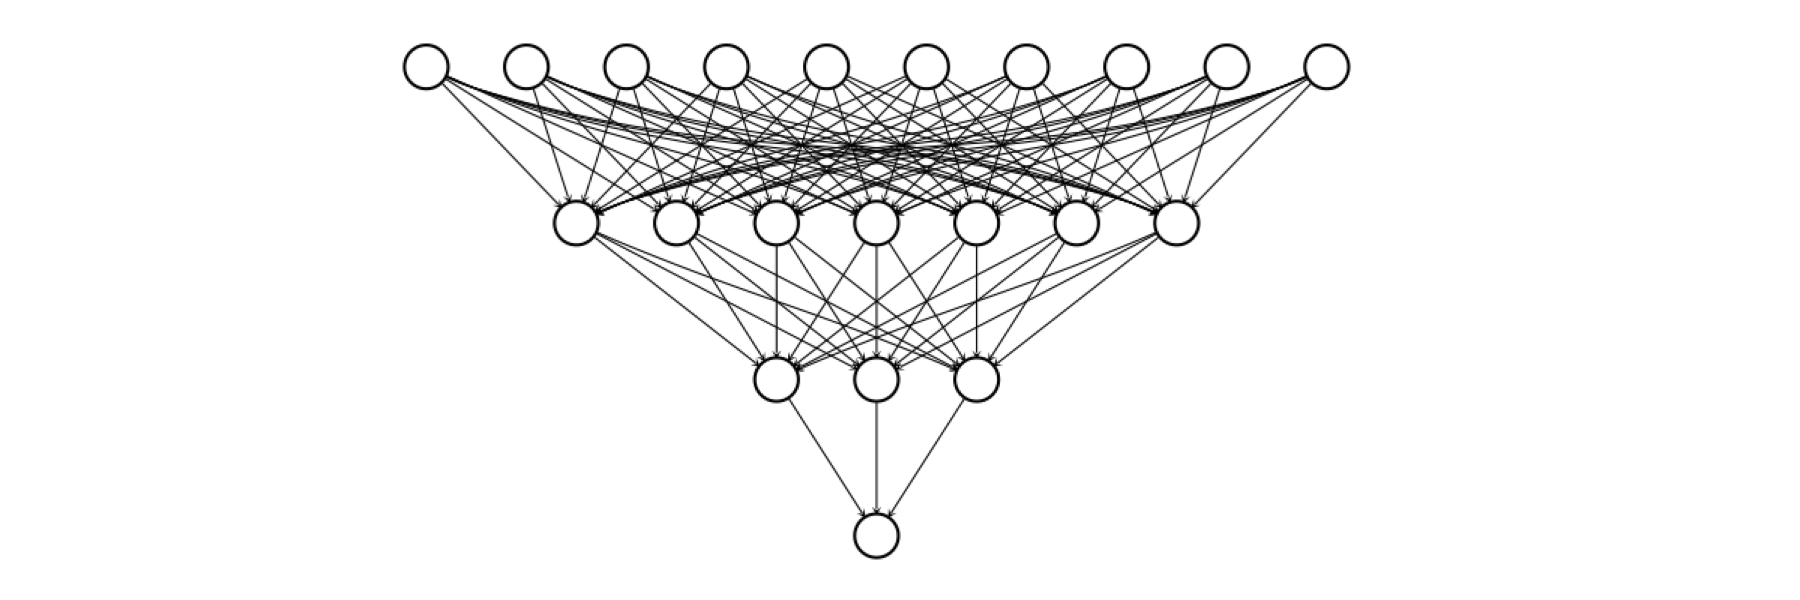
\includegraphics{../Figures/6. Using the dense layer operation.png}
\caption{Using the dense layer operation}
\end{figure}

    \(\blacktriangleright\) \textbf{Package pre-loading}

    \begin{tcolorbox}[breakable, size=fbox, boxrule=1pt, pad at break*=1mm,colback=cellbackground, colframe=cellborder]
\prompt{In}{incolor}{8}{\boxspacing}
\begin{Verbatim}[commandchars=\\\{\}]
\PY{k+kn}{import} \PY{n+nn}{pandas} \PY{k}{as} \PY{n+nn}{pd}
\end{Verbatim}
\end{tcolorbox}

    \(\blacktriangleright\) \textbf{Data pre-loading}

    \begin{tcolorbox}[breakable, size=fbox, boxrule=1pt, pad at break*=1mm,colback=cellbackground, colframe=cellborder]
\prompt{In}{incolor}{9}{\boxspacing}
\begin{Verbatim}[commandchars=\\\{\}]
\PY{n}{df} \PY{o}{=} \PY{n}{pd}\PY{o}{.}\PY{n}{read\PYZus{}csv}\PY{p}{(}\PY{l+s+s2}{\PYZdq{}}\PY{l+s+s2}{../Datasets/1. Borrower features.csv}\PY{l+s+s2}{\PYZdq{}}\PY{p}{,} \PY{n}{header}\PY{o}{=}\PY{k+kc}{None}\PY{p}{)}
\PY{n}{borrower\PYZus{}features} \PY{o}{=} \PY{n}{constant}\PY{p}{(}\PY{n}{df}\PY{p}{,} \PY{n}{dtype}\PY{o}{=}\PY{n}{float32}\PY{p}{)}
\end{Verbatim}
\end{tcolorbox}

    \(\blacktriangleright\) \textbf{Task practice}

    \begin{tcolorbox}[breakable, size=fbox, boxrule=1pt, pad at break*=1mm,colback=cellbackground, colframe=cellborder]
\prompt{In}{incolor}{10}{\boxspacing}
\begin{Verbatim}[commandchars=\\\{\}]
\PY{c+c1}{\PYZsh{} Define the first dense layer}
\PY{n}{dense1} \PY{o}{=} \PY{n}{keras}\PY{o}{.}\PY{n}{layers}\PY{o}{.}\PY{n}{Dense}\PY{p}{(}\PY{l+m+mi}{7}\PY{p}{,} \PY{n}{activation}\PY{o}{=}\PY{l+s+s1}{\PYZsq{}}\PY{l+s+s1}{sigmoid}\PY{l+s+s1}{\PYZsq{}}\PY{p}{)}\PY{p}{(}\PY{n}{borrower\PYZus{}features}\PY{p}{)}

\PY{c+c1}{\PYZsh{} Define a dense layer with 3 output nodes}
\PY{n}{dense2} \PY{o}{=} \PY{n}{keras}\PY{o}{.}\PY{n}{layers}\PY{o}{.}\PY{n}{Dense}\PY{p}{(}\PY{l+m+mi}{3}\PY{p}{,} \PY{n}{activation}\PY{o}{=}\PY{l+s+s1}{\PYZsq{}}\PY{l+s+s1}{sigmoid}\PY{l+s+s1}{\PYZsq{}}\PY{p}{)}\PY{p}{(}\PY{n}{dense1}\PY{p}{)}

\PY{c+c1}{\PYZsh{} Define a dense layer with 1 output node}
\PY{n}{predictions} \PY{o}{=} \PY{n}{keras}\PY{o}{.}\PY{n}{layers}\PY{o}{.}\PY{n}{Dense}\PY{p}{(}\PY{l+m+mi}{1}\PY{p}{,} \PY{n}{activation}\PY{o}{=}\PY{l+s+s1}{\PYZsq{}}\PY{l+s+s1}{sigmoid}\PY{l+s+s1}{\PYZsq{}}\PY{p}{)}\PY{p}{(}\PY{n}{dense2}\PY{p}{)}

\PY{c+c1}{\PYZsh{} Print the shapes of dense1, dense2, and predictions}
\PY{n+nb}{print}\PY{p}{(}\PY{l+s+s1}{\PYZsq{}}\PY{l+s+se}{\PYZbs{}n}\PY{l+s+s1}{ shape of dense1: }\PY{l+s+s1}{\PYZsq{}}\PY{p}{,} \PY{n}{dense1}\PY{o}{.}\PY{n}{shape}\PY{p}{)}
\PY{n+nb}{print}\PY{p}{(}\PY{l+s+s1}{\PYZsq{}}\PY{l+s+se}{\PYZbs{}n}\PY{l+s+s1}{ shape of dense2: }\PY{l+s+s1}{\PYZsq{}}\PY{p}{,} \PY{n}{dense2}\PY{o}{.}\PY{n}{shape}\PY{p}{)}
\PY{n+nb}{print}\PY{p}{(}\PY{l+s+s1}{\PYZsq{}}\PY{l+s+se}{\PYZbs{}n}\PY{l+s+s1}{ shape of predictions: }\PY{l+s+s1}{\PYZsq{}}\PY{p}{,} \PY{n}{predictions}\PY{o}{.}\PY{n}{shape}\PY{p}{)}
\end{Verbatim}
\end{tcolorbox}

    \begin{Verbatim}[commandchars=\\\{\}]

 shape of dense1:  (100, 7)

 shape of dense2:  (100, 3)

 shape of predictions:  (100, 1)
    \end{Verbatim}

    \begin{tcolorbox}[breakable, size=fbox, boxrule=1pt, pad at break*=1mm,colback=cellbackground, colframe=cellborder]
\prompt{In}{incolor}{34}{\boxspacing}
\begin{Verbatim}[commandchars=\\\{\}]
\PY{k+kn}{import} \PY{n+nn}{tensorflow}
\end{Verbatim}
\end{tcolorbox}

    \begin{tcolorbox}[breakable, size=fbox, boxrule=1pt, pad at break*=1mm,colback=cellbackground, colframe=cellborder]
\prompt{In}{incolor}{38}{\boxspacing}
\begin{Verbatim}[commandchars=\\\{\}]
\PY{n}{dense} \PY{o}{=} \PY{n}{tensorflow}\PY{o}{.}\PY{n}{keras}\PY{o}{.}\PY{n}{layers}\PY{o}{.}\PY{n}{Dense}\PY{p}{(}\PY{l+m+mi}{10}\PY{p}{,} \PY{n}{activation}\PY{o}{=}\PY{l+s+s1}{\PYZsq{}}\PY{l+s+s1}{sigmoid}\PY{l+s+s1}{\PYZsq{}}\PY{p}{)}\PY{p}{(}\PY{n}{dense2}\PY{p}{)}
\end{Verbatim}
\end{tcolorbox}

    \begin{tcolorbox}[breakable, size=fbox, boxrule=1pt, pad at break*=1mm,colback=cellbackground, colframe=cellborder]
\prompt{In}{incolor}{39}{\boxspacing}
\begin{Verbatim}[commandchars=\\\{\}]
\PY{n}{dense}\PY{o}{.}\PY{n}{shape}
\end{Verbatim}
\end{tcolorbox}

            \begin{tcolorbox}[breakable, size=fbox, boxrule=.5pt, pad at break*=1mm, opacityfill=0]
\prompt{Out}{outcolor}{39}{\boxspacing}
\begin{Verbatim}[commandchars=\\\{\}]
TensorShape([100, 10])
\end{Verbatim}
\end{tcolorbox}
        
    \begin{tcolorbox}[breakable, size=fbox, boxrule=1pt, pad at break*=1mm,colback=cellbackground, colframe=cellborder]
\prompt{In}{incolor}{40}{\boxspacing}
\begin{Verbatim}[commandchars=\\\{\}]
\PY{n}{dense2}\PY{o}{.}\PY{n}{shape}
\end{Verbatim}
\end{tcolorbox}

            \begin{tcolorbox}[breakable, size=fbox, boxrule=.5pt, pad at break*=1mm, opacityfill=0]
\prompt{Out}{outcolor}{40}{\boxspacing}
\begin{Verbatim}[commandchars=\\\{\}]
TensorShape([100, 5])
\end{Verbatim}
\end{tcolorbox}
        
    \begin{tcolorbox}[breakable, size=fbox, boxrule=1pt, pad at break*=1mm,colback=cellbackground, colframe=cellborder]
\prompt{In}{incolor}{ }{\boxspacing}
\begin{Verbatim}[commandchars=\\\{\}]

\end{Verbatim}
\end{tcolorbox}

    \begin{tcolorbox}[breakable, size=fbox, boxrule=1pt, pad at break*=1mm,colback=cellbackground, colframe=cellborder]
\prompt{In}{incolor}{ }{\boxspacing}
\begin{Verbatim}[commandchars=\\\{\}]

\end{Verbatim}
\end{tcolorbox}

    \begin{tcolorbox}[breakable, size=fbox, boxrule=1pt, pad at break*=1mm,colback=cellbackground, colframe=cellborder]
\prompt{In}{incolor}{ }{\boxspacing}
\begin{Verbatim}[commandchars=\\\{\}]

\end{Verbatim}
\end{tcolorbox}

    \begin{tcolorbox}[breakable, size=fbox, boxrule=1pt, pad at break*=1mm,colback=cellbackground, colframe=cellborder]
\prompt{In}{incolor}{ }{\boxspacing}
\begin{Verbatim}[commandchars=\\\{\}]

\end{Verbatim}
\end{tcolorbox}

    \begin{tcolorbox}[breakable, size=fbox, boxrule=1pt, pad at break*=1mm,colback=cellbackground, colframe=cellborder]
\prompt{In}{incolor}{ }{\boxspacing}
\begin{Verbatim}[commandchars=\\\{\}]

\end{Verbatim}
\end{tcolorbox}

    \begin{tcolorbox}[breakable, size=fbox, boxrule=1pt, pad at break*=1mm,colback=cellbackground, colframe=cellborder]
\prompt{In}{incolor}{ }{\boxspacing}
\begin{Verbatim}[commandchars=\\\{\}]

\end{Verbatim}
\end{tcolorbox}

    \hypertarget{requirements}{%
\section{Requirements}\label{requirements}}

    \begin{tcolorbox}[breakable, size=fbox, boxrule=1pt, pad at break*=1mm,colback=cellbackground, colframe=cellborder]
\prompt{In}{incolor}{ }{\boxspacing}
\begin{Verbatim}[commandchars=\\\{\}]
\PY{k+kn}{from} \PY{n+nn}{platform} \PY{k+kn}{import} \PY{n}{python\PYZus{}version}
\PY{k+kn}{import} \PY{n+nn}{sklearn}

\PY{n}{python\PYZus{}version} \PY{o}{=} \PY{p}{(}\PY{l+s+s1}{\PYZsq{}}\PY{l+s+s1}{python==}\PY{l+s+si}{\PYZob{}\PYZcb{}}\PY{l+s+s1}{\PYZsq{}}\PY{o}{.}\PY{n}{format}\PY{p}{(}\PY{n}{python\PYZus{}version}\PY{p}{(}\PY{p}{)}\PY{p}{)}\PY{p}{)}
\PY{n}{numpy\PYZus{}version} \PY{o}{=} \PY{p}{(}\PY{l+s+s1}{\PYZsq{}}\PY{l+s+s1}{numpy==}\PY{l+s+si}{\PYZob{}\PYZcb{}}\PY{l+s+s1}{\PYZsq{}}\PY{o}{.}\PY{n}{format}\PY{p}{(}\PY{n}{np}\PY{o}{.}\PY{n}{\PYZus{}\PYZus{}version\PYZus{}\PYZus{}}\PY{p}{)}\PY{p}{)}
\PY{n}{pandas\PYZus{}version} \PY{o}{=} \PY{p}{(}\PY{l+s+s1}{\PYZsq{}}\PY{l+s+s1}{pandas==}\PY{l+s+si}{\PYZob{}\PYZcb{}}\PY{l+s+s1}{\PYZsq{}}\PY{o}{.}\PY{n}{format}\PY{p}{(}\PY{n}{pd}\PY{o}{.}\PY{n}{\PYZus{}\PYZus{}version\PYZus{}\PYZus{}}\PY{p}{)}\PY{p}{)}
\PY{n}{tensorflow\PYZus{}version} \PY{o}{=} \PY{p}{(}\PY{l+s+s1}{\PYZsq{}}\PY{l+s+s1}{tensorflow==}\PY{l+s+si}{\PYZob{}\PYZcb{}}\PY{l+s+s1}{\PYZsq{}}\PY{o}{.}\PY{n}{format}\PY{p}{(}\PY{n}{tf}\PY{o}{.}\PY{n}{\PYZus{}\PYZus{}version\PYZus{}\PYZus{}}\PY{p}{)}\PY{p}{)}
\PY{n}{scikit\PYZus{}learn\PYZus{}version} \PY{o}{=} \PY{p}{(}\PY{l+s+s1}{\PYZsq{}}\PY{l+s+s1}{scikit\PYZhy{}learn==}\PY{l+s+si}{\PYZob{}\PYZcb{}}\PY{l+s+s1}{\PYZsq{}}\PY{o}{.}\PY{n}{format}\PY{p}{(}\PY{n}{sklearn}\PY{o}{.}\PY{n}{\PYZus{}\PYZus{}version\PYZus{}\PYZus{}}\PY{p}{)}\PY{p}{)}

\PY{n}{writepath} \PY{o}{=} \PY{l+s+s1}{\PYZsq{}}\PY{l+s+s1}{../../requirements.txt}\PY{l+s+s1}{\PYZsq{}}
\PY{n}{requirements} \PY{o}{=} \PY{p}{[}\PY{p}{]}
\PY{n}{packages} \PY{o}{=} \PY{p}{[}
    \PY{n}{numpy\PYZus{}version}\PY{p}{,} \PY{n}{pandas\PYZus{}version}\PY{p}{,} \PY{n}{tensorflow\PYZus{}version}\PY{p}{,} \PY{n}{scikit\PYZus{}learn\PYZus{}version}
\PY{p}{]}

\PY{k}{try}\PY{p}{:}
    \PY{k}{with} \PY{n+nb}{open}\PY{p}{(}\PY{n}{writepath}\PY{p}{,} \PY{l+s+s1}{\PYZsq{}}\PY{l+s+s1}{r+}\PY{l+s+s1}{\PYZsq{}}\PY{p}{)} \PY{k}{as} \PY{n}{file}\PY{p}{:}
        \PY{k}{for} \PY{n}{line} \PY{o+ow}{in} \PY{n}{file}\PY{p}{:}
            \PY{n}{requirements}\PY{o}{.}\PY{n}{append}\PY{p}{(}\PY{n}{line}\PY{o}{.}\PY{n}{strip}\PY{p}{(}\PY{l+s+s1}{\PYZsq{}}\PY{l+s+se}{\PYZbs{}n}\PY{l+s+s1}{\PYZsq{}}\PY{p}{)}\PY{p}{)}
\PY{k}{except}\PY{p}{:}
    \PY{k}{with} \PY{n+nb}{open}\PY{p}{(}\PY{n}{writepath}\PY{p}{,} \PY{l+s+s1}{\PYZsq{}}\PY{l+s+s1}{w+}\PY{l+s+s1}{\PYZsq{}}\PY{p}{)} \PY{k}{as} \PY{n}{file}\PY{p}{:}
        \PY{k}{for} \PY{n}{line} \PY{o+ow}{in} \PY{n}{file}\PY{p}{:}
            \PY{n}{requirements}\PY{o}{.}\PY{n}{append}\PY{p}{(}\PY{n}{line}\PY{o}{.}\PY{n}{strip}\PY{p}{(}\PY{l+s+s1}{\PYZsq{}}\PY{l+s+se}{\PYZbs{}n}\PY{l+s+s1}{\PYZsq{}}\PY{p}{)}\PY{p}{)}

\PY{k}{with} \PY{n+nb}{open}\PY{p}{(}\PY{n}{writepath}\PY{p}{,} \PY{l+s+s1}{\PYZsq{}}\PY{l+s+s1}{a}\PY{l+s+s1}{\PYZsq{}}\PY{p}{)} \PY{k}{as} \PY{n}{file}\PY{p}{:}
    \PY{k}{for} \PY{n}{package} \PY{o+ow}{in} \PY{n}{packages}\PY{p}{:}
        \PY{k}{if} \PY{n}{package} \PY{o+ow}{not} \PY{o+ow}{in} \PY{n}{requirements}\PY{p}{:}
            \PY{n}{file}\PY{o}{.}\PY{n}{write}\PY{p}{(}\PY{n}{package} \PY{o}{+} \PY{l+s+s1}{\PYZsq{}}\PY{l+s+se}{\PYZbs{}n}\PY{l+s+s1}{\PYZsq{}}\PY{p}{)}

\PY{n}{max\PYZus{}characters} \PY{o}{=} \PY{n+nb}{len}\PY{p}{(}\PY{n}{python\PYZus{}version}\PY{p}{)}
\PY{k}{for} \PY{n}{package} \PY{o+ow}{in} \PY{n}{packages}\PY{p}{:}
    \PY{k}{if} \PY{n+nb}{max}\PY{p}{(}\PY{n}{max\PYZus{}characters}\PY{p}{,} \PY{n+nb}{len}\PY{p}{(}\PY{n}{package}\PY{p}{)}\PY{p}{)} \PY{o}{\PYZgt{}} \PY{n}{max\PYZus{}characters}\PY{p}{:}
        \PY{n}{max\PYZus{}characters} \PY{o}{=} \PY{n+nb}{max}\PY{p}{(}\PY{n}{max\PYZus{}characters}\PY{p}{,} \PY{n+nb}{len}\PY{p}{(}\PY{n}{package}\PY{p}{)}\PY{p}{)}

\PY{n+nb}{print}\PY{p}{(}\PY{l+s+s1}{\PYZsq{}}\PY{l+s+s1}{\PYZsh{}}\PY{l+s+s1}{\PYZsq{}} \PY{o}{*} \PY{p}{(}\PY{n}{max\PYZus{}characters} \PY{o}{+} \PY{l+m+mi}{8}\PY{p}{)}\PY{p}{)}
\PY{n+nb}{print}\PY{p}{(}\PY{l+s+s1}{\PYZsq{}}\PY{l+s+s1}{\PYZsh{}}\PY{l+s+s1}{\PYZsq{}} \PY{o}{*} \PY{l+m+mi}{2} \PY{o}{+} \PY{l+s+s1}{\PYZsq{}}\PY{l+s+s1}{ }\PY{l+s+s1}{\PYZsq{}} \PY{o}{*} \PY{p}{(}\PY{n}{max\PYZus{}characters} \PY{o}{+} \PY{l+m+mi}{4}\PY{p}{)} \PY{o}{+} \PY{l+s+s1}{\PYZsq{}}\PY{l+s+s1}{\PYZsh{}}\PY{l+s+s1}{\PYZsq{}} \PY{o}{*} \PY{l+m+mi}{2}\PY{p}{)}
\PY{n+nb}{print}\PY{p}{(}\PY{l+s+s1}{\PYZsq{}}\PY{l+s+s1}{\PYZsh{}}\PY{l+s+s1}{\PYZsq{}} \PY{o}{*} \PY{l+m+mi}{2} \PY{o}{+} \PY{l+s+s1}{\PYZsq{}}\PY{l+s+s1}{ }\PY{l+s+s1}{\PYZsq{}} \PY{o}{*} \PY{l+m+mi}{2} \PY{o}{+} \PY{n}{python\PYZus{}version} \PY{o}{+} \PY{l+s+s1}{\PYZsq{}}\PY{l+s+s1}{ }\PY{l+s+s1}{\PYZsq{}} \PY{o}{*}
      \PY{p}{(}\PY{n}{max\PYZus{}characters} \PY{o}{\PYZhy{}} \PY{n+nb}{len}\PY{p}{(}\PY{n}{python\PYZus{}version}\PY{p}{)} \PY{o}{+} \PY{l+m+mi}{2}\PY{p}{)} \PY{o}{+} \PY{l+s+s1}{\PYZsq{}}\PY{l+s+s1}{\PYZsh{}}\PY{l+s+s1}{\PYZsq{}} \PY{o}{*} \PY{l+m+mi}{2}\PY{p}{)}
\PY{k}{for} \PY{n}{package} \PY{o+ow}{in} \PY{n}{packages}\PY{p}{:}
    \PY{n+nb}{print}\PY{p}{(}\PY{l+s+s1}{\PYZsq{}}\PY{l+s+s1}{\PYZsh{}}\PY{l+s+s1}{\PYZsq{}} \PY{o}{*} \PY{l+m+mi}{2} \PY{o}{+} \PY{l+s+s1}{\PYZsq{}}\PY{l+s+s1}{ }\PY{l+s+s1}{\PYZsq{}} \PY{o}{*} \PY{l+m+mi}{2} \PY{o}{+} \PY{n}{package} \PY{o}{+} \PY{l+s+s1}{\PYZsq{}}\PY{l+s+s1}{ }\PY{l+s+s1}{\PYZsq{}} \PY{o}{*}
          \PY{p}{(}\PY{n}{max\PYZus{}characters} \PY{o}{\PYZhy{}} \PY{n+nb}{len}\PY{p}{(}\PY{n}{package}\PY{p}{)} \PY{o}{+} \PY{l+m+mi}{2}\PY{p}{)} \PY{o}{+} \PY{l+s+s1}{\PYZsq{}}\PY{l+s+s1}{\PYZsh{}}\PY{l+s+s1}{\PYZsq{}} \PY{o}{*} \PY{l+m+mi}{2}\PY{p}{)}
\PY{n+nb}{print}\PY{p}{(}\PY{l+s+s1}{\PYZsq{}}\PY{l+s+s1}{\PYZsh{}}\PY{l+s+s1}{\PYZsq{}} \PY{o}{*} \PY{l+m+mi}{2} \PY{o}{+} \PY{l+s+s1}{\PYZsq{}}\PY{l+s+s1}{ }\PY{l+s+s1}{\PYZsq{}} \PY{o}{*} \PY{p}{(}\PY{n}{max\PYZus{}characters} \PY{o}{+} \PY{l+m+mi}{4}\PY{p}{)} \PY{o}{+} \PY{l+s+s1}{\PYZsq{}}\PY{l+s+s1}{\PYZsh{}}\PY{l+s+s1}{\PYZsq{}} \PY{o}{*} \PY{l+m+mi}{2}\PY{p}{)}
\PY{n+nb}{print}\PY{p}{(}\PY{l+s+s1}{\PYZsq{}}\PY{l+s+s1}{\PYZsh{}}\PY{l+s+s1}{\PYZsq{}} \PY{o}{*} \PY{p}{(}\PY{n}{max\PYZus{}characters} \PY{o}{+} \PY{l+m+mi}{8}\PY{p}{)}\PY{p}{)}
\end{Verbatim}
\end{tcolorbox}


    % Add a bibliography block to the postdoc
    
    
    
\end{document}
